\subsection*{\underline{Funcionalidade adicionada}:}

Buscando por \texttt{issues} no GitHub, encontramos um
\href{https://github.com/pixelated-project/pixelated-user-agent/issues/}
{bugtracker} bastante organizado, com tags para
diferentes estágios de desenvolvimento (backlog, ready, development, etc),
áreas de desenvolvimento (design, encryption, etc) e dificuldade (beginners).

A \texttt{issue} escolhida foi a seguinte:
\href{https://github.com/pixelated-project/pixelated-user-agent/issues/384}
{``Keep input label always present when composing an email''}. Resumindo, pede-se
para implementar
\href{http://bradfrost.com/blog/post/float-label-pattern}{float labels} tanto para o
Subject quanto para o Body na hora de compôr uma mensagem/editar um rascunho.

Apesar de ser uma feature pequena, ela nos exigiu muitas horas de \texttt{hacking} pois
precisamos entender a estrutura do código do Pixelated para saber onde fazer as
modificações. Tivemos que alterar o HTML, o CSS e o Javascript das seções de
composição do email e alteramos, no total, 4 arquivos.

\begin{figure}[h]
\centering
\begin{subfigure}{.5\textwidth}
  \centering
  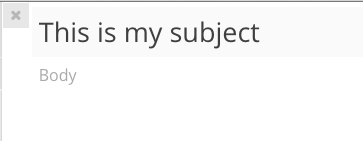
\includegraphics[width=.75\linewidth]{src/issue1.png}
\end{subfigure}%
\begin{subfigure}{.5\textwidth}
  \centering
  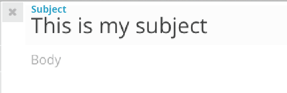
\includegraphics[width=.9\linewidth]{src/issue2.png}
\end{subfigure}
\caption*{Esboço da funcionalidade}
\end{figure}

Primeiramente nos preocupamos simplesmente em fazer a feature funcionar.
Nesse passo, tivemos dificuldade com o código Javascript pois ele
possui uma estrutura bastante complexa no Pixelated e nenhum dos integrantes do
grupo tinha experiência com a organização de código de front-end.

Depois, com a funcionalidade pronta, refatoramos o código para organizá-lo
corretamente e melhorar sua qualidade antes de submetê-lo para o repositório oficial.

O processo de submissão foi bem simples. Os passos foram os seguintes:
  \begin{itemize}
    \item Fizemos um fork do repositório oficial no GitHub.
    \item Clonamos esse fork para a nossa máquina.
    \item Criamos uma branch local.
    \item Fizemos um commit com o código da funcionalidade.
    \item Subimos esse commit para a branch separada no nosso repositório remoto.
    \item Fizemos um pull request da branch de trabalho do nosso repositório
    para a branch master do repositório oficial.
  \end{itemize}

Como já dito anteriormente, recebemos feedback logo em seguida, em questão de
minutos, com sugestões de melhorias para o código como renomear um seletor CSS
e mover uma função Javascript para o arquivo correto. Não houve tempo suficiente
para fazer aplicarmos essas alterações antes da escrita desse relatório, mas
as implementaremos assim que possível para que nossa contribuição seja incluída
no Pixelated.